\documentclass{nime-alternate}
\usepackage{listings}
\begin{document}

%\conferenceinfo{NIME'18,}{June 3-6, 2018, Blacksburg, Virginia, USA.}
\title{A SPECTRAL EXPERIENCE: SELF CONVOLUTION AND FACE TRACKING}

\author{Federico Camara Halac\\\affaddr{NYU}\\\affaddr{New York, USA}\\\email{fch226@nyu.edu}}
% For your initial submission you MUST ANONYMIZE the authors.
\newcommand{\ttt}{\raise.17ex\hbox{$\scriptstyle\mathtt{\sim}$}}
\maketitle

\begin{abstract}
 ``Hearing The Self: A Spectral Experience'' (aka HALLY) is an interactive, immersive, multimedia, and robotic installation, simulating the process by which the human brain perceives the world. This paper explores the role of both sound and image in the definition of the self this installation brings forth. We briefly explore previous approaches to image sonification, and propose that through video-based convolution new conceptualizations of the self can arise. Further, this expression of the self is neither centered on the human participant nor on the socially constructed notions of the self, but on nonhuman aspects such as the reflection and capture of light, or the technological array of the installation as such. The participant's exploration within this spectrality results in an uncanny and playful experience.
\end{abstract}
\keywords{Interactive, immersive, multimedia, installation, sonification, spatialization, nonhuman self}

\section{Introduction}
\textit{``Spectrality is nonhumans, including the 'nonhuman' aspect of ourselves.''} Timothy Morton, (p.54) \cite{morton:humankind}
%

HALLY\footnote{This installation is a collaboration between Lucia Dora Simonelli (ICTP) in Trieste, Italy, Matias Gonzalo Delgadino (Imperial College) in London, UK, and Federico Camara Halac (NYU) in New York, USA. It was premiered in the Xuhui Art Museum, Shanghai, China, during the International Computer Music Conference, October 2017. The source code is available here: \url{https://fdch.github.io/specexp/}. A short video is available here: \url{https://vimeo.com/241401699}} consists of a pitch-black room surrounded with speakers, two screens on the front, a camera-hacked mic stand, a sustain pedal, and a delineated square on the floor delimiting the capturing area. The experience begins when the participant enters the room and her face is detected in the capturing area, triggering a random scene. 

This installation simultaneously addresses that the mechanical process by which the human brain perceives the world, i.e. the Inverse Fourier Transform (IFT) component of perception, even when perceiving one's own self, is only a part of a complex process shaped by many external stimuli, one of the strongest being societal. However, as we attempt to show, nonhuman agency is essential to the definition of self proposed here.

The remainder of this document is concerned with showing previous experiments on image sonification, the mechanics of the installation, the aesthetic opportunities that were explored, and a brief discussion on the type of questions that emerged from this experience of the self.

\section{Image sonification}

In opposition to (data) visualization, the temporal nature of sound favors at least three musical qualities. First, the detection of \textit{patterns} and \textit{trends}, understood as salient information from multidimensional data\cite{bental:sonification,bental:sonification2}, generally approached from a \textit{parameter-mapping} perspective\cite{kramer:principles,bental:sonart,yeo:framework}, and ultimately arriving at \textit{raster sonification}\cite{yeo:raster}. Second, the construction of a sequential \textit{narrative of emotion} (i.e., physical properties, visceral information), that is available through sound \cite{polli:sonification}. Third, more recent research in spatialization has led to sound installations, with variable degrees of interactivity, which convey spatial data sonification\cite{weinberg:brainwaves}. 

On one hand, previous work on the conversion of images to sound patterns aimed towards a hearing aid for the sight impaired\cite{meijer:auditory}. Although this is the first portable, real-time system that translates image information, its usefulness depends on its scientific accuracy. On the other hand, composers have tended towards \textit{musical} data sonification, i.e. without the need for conveying useful information\cite{bental:sonification,bental:sonification2}. To a certain extent, the mathematical preservation of information can be understood as a mid-term in this conjunction\cite{thiebaut:images}. 

Thus, in our present installation we are conveying a scientifically useless, but mathematically equivalent sonification of a bi-dimensional array containing a constantly updated, gray-scale image, in order to bring into experience the physicality of spatialized sound.


\section{Mechanics}
From a mechanical point of view, it has been suggested that the human brain is a machine that performs an IFT through which it constructs a geometric image from correlations of reflections of light.\cite{connes:shapes} (Visual) perception can be therefore visualized with an image sensor and a Fast Fourier Transform (FFT) computation of the image data.\cite{camara:pixfft2} Furthermore, image data (i.e., a large array of values) can filter a given sound signal of the same length. In Pure Data\cite{puckette:puredata} (Pd), if the block (the DSP array) size matches the length of the image array, a video-based convolution is possible in real time. Thus, by filtering uniform noise with the 2d FFT of an image stream we arrive at a sonification of the mechanics of the human brain's perception within the context of an interactive, real time installation. 


\begin{figure}[htbp]
    \centering
        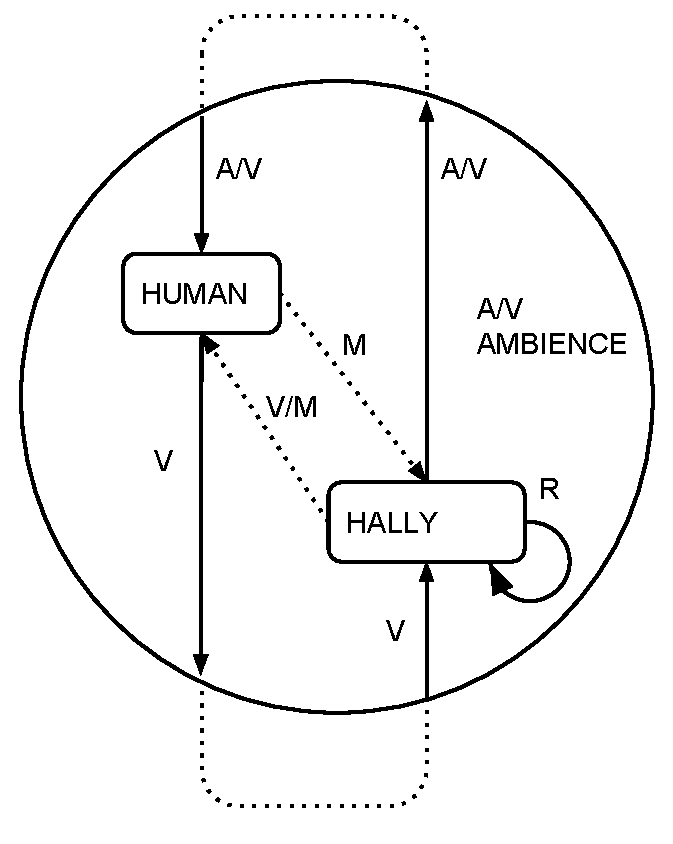
\includegraphics[width=1\columnwidth]{hally-human-1}
    \caption{Adapted from Di Scipio's triangular recursive ecosystem connection \cite{discipio:interface}. A: audio; V: visual; M: motility; R: randomness}
    \label{fig:hally-human-1}
\end{figure}

\subsection{[pix\_fft2]}
\label{sec:2dfft}
The two-dimensional FFT computation of the image array was implemented in a custom external for Gem\cite{danks:gem}, using the FFTW\footnote{\url{http://fftw.org}} library. This approach, as opposed to the already existing pix\_opencv\_dft, was taken namely because of speed -the FFTW algorithms are faster\footnote{\url{http://www.fftw.org/speed}} than the native OpenCV Discrete Fourier Transform\footnote{\url{https://docs.opencv.org/2.4/modules/core/doc/operations_on_arrays.html\#dft}} (DFT) routine- and flexibility regarding future development. Speed in FFTW is dependent upon fixed memory allocation, which became a integral part of the installation in the sense that the computed area of the image was always of the same size (128x128), and remained as such throughout the three days of the performance. Further development of a more embracing Pd object wrapping FFTW would be of interest, particularly in dealing with multi-dimensional FFT computation. 

\subsection{Face Tracking and repositioning}
\label{sec:facetracking}
Antoine Villeret's pix\_opencv library\footnote{\url{https://github.com/avilleret/pix\_opencv}} includes another library called FaceTracker\cite{sarahig:facetracker}  (from here on FT) which performs face detection and tracking by deformable model fitting (i.e., a face mesh). Given that the  size of the image was of 640x480, we could adjust the center position of the face to a box of 128x128 pixels. Thus, by repositioning within the larger image according to the position of the participant within the capturing area, we obtained a responsive surveillance system that constantly looks and follows around the participant's face. Furthermore, the \textit{scenes} that occur throughout the installation are triggered by a sudden face detection. Therefore, when idle, HALLY is computing dark frames looking for shapes to match the FT's mesh. When a mesh is detected, HALLY triggers a random scene.

The weakness of this approach is first the extensive computation that is constantly required to find a face. The second weakness is that, though rarely, dim light conditions and possible occlusions to the face, as well as figures that may resemble a face (e.g. a speaker in the back of the room) make human faces pass undetected. On the one hand, the expensive computations had no effect on the performance of the installation, neither on the Laptop Computer (LC) where FT was called from pix\_open\_cv (i.e., from Pd), nor on the RPI 3, where the FT demo was running, modified to only send the resulting mesh via TCP/IP through Ethernet to the LC. On the other hand, the problem of the undetected face raised other issues, such as the meaning of the face itself, in relation to the self as such. This last philosophical question we leave to the reader to wonder, much in the same way the participant is left with a similar questioning, regarding the difference of her own self to that of the other.

\begin{figure}[htbp]
    \centering
        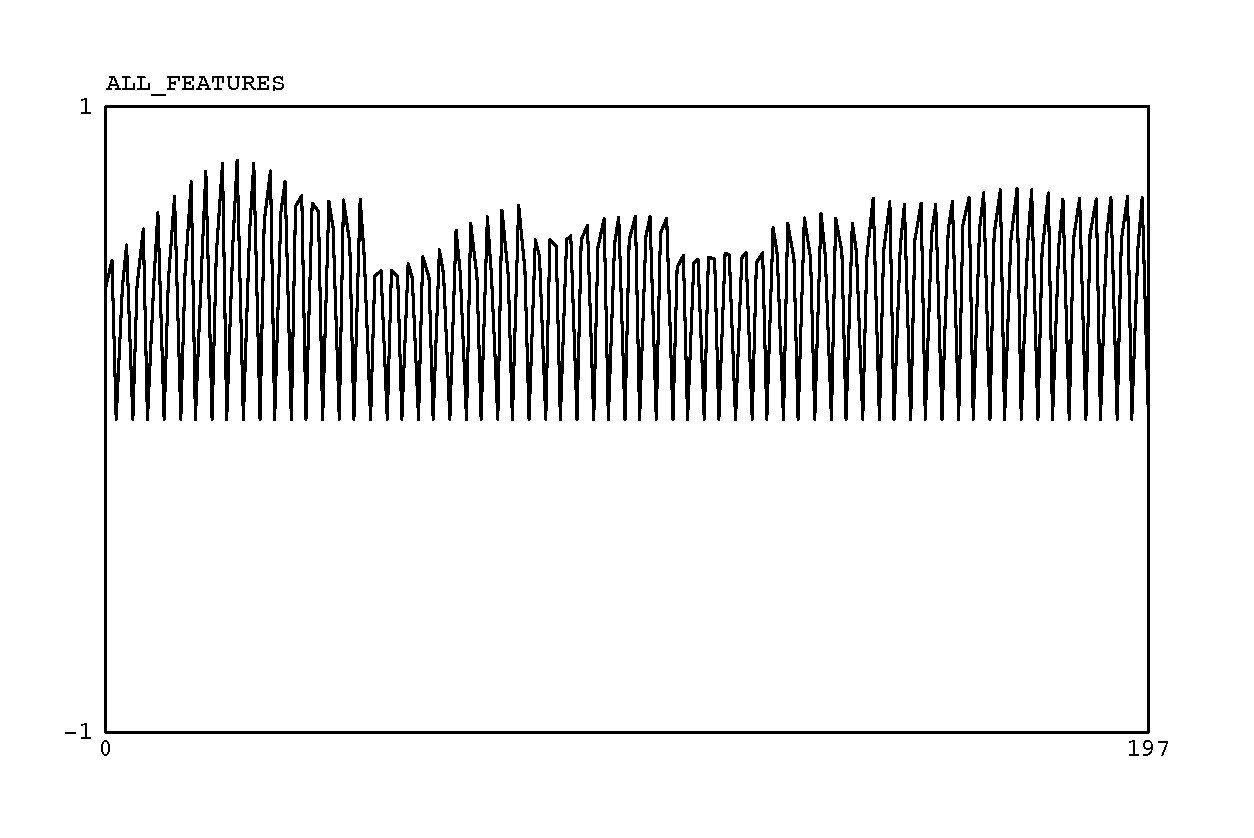
\includegraphics[width=1\columnwidth]{ALL_FEATURES}
    \caption{Array holding the 198 points of the face mesh, as determined by the FaceTracker library.}
    \label{fig:ALL_FEATURES}
\end{figure}

\subsection{Mimicking tilt gesture }
\label{sec:mimicking}
This is an inherently physical aspect of HALLY: the two image sensors are aligned so that they resemble a face with two eyes. Given that both sensors are screwed to the plastic part of a microphone stand which adjusts the angle of the top microphone's arm (removed for the purposes of this installation), HALLY's face has the ability to tilt +15 or -15 degrees in the z-axis. With the aid of a string attached to a servo motor at the bottom of the microphone stand, this tilt is performed automatically with an Arduino (UNO) that is receiving impulses via USB from the LC and interpreting them as -15 or +15 degrees of tilting. In turn, these impulses are triggered by analyzing the angle of the four points assigned to the nose in the FT's face mesh. 

The above results in a mirrored responsive gesture on the part of HALLY: if the participant's nose is tilted to the right, HALLY will tilt to the left, and vice-versa. However, if the participant's face is exactly aligned at 0 degrees, then HALLY will turn randomly left and right in a feedback loop: the tilting rotates the image sensor by +15, so it sends an impulse to adjust -15, and then it has to rotate back to +15 degrees, etc. This feedback loop is ongoing until the participant mimics the gesture as well, therefore exiting the loop.\footnote{The macrame string that provided this mechanic motion was hardly ever properly adjusted, so it often happened that it detached. Notwithstanding, this un-working of the installation was left as such, since we considered it a very small but delicate attention on our side to aid HALLY, and it constituted a break into the reality of the technologies involved. } The sonic repercussions were audible, since the entire image captured was rotated (by a small amount), and therefore the pixel values shifted places changing the shape of the convolution. This mimicking gesture is a brief but uncanny quality that HALLY brings forth, not only because it resembles a human gesture, but also because it places the non-human and the human in the same feedback loop, therefore providing both with the same resonance in listening\footnote{This installation's first part of the name ``Hearing the Self...'' originally came from the theme of the ICMC where it was performed. The hearing of the self remains as such only if you pass by the installation space, hearing a low drone or a very active and loud sound space; if you go through the curtains, though -only when entering- , the listening of the self takes place.} the self.

\begin{figure}[htbp]
    \centering
        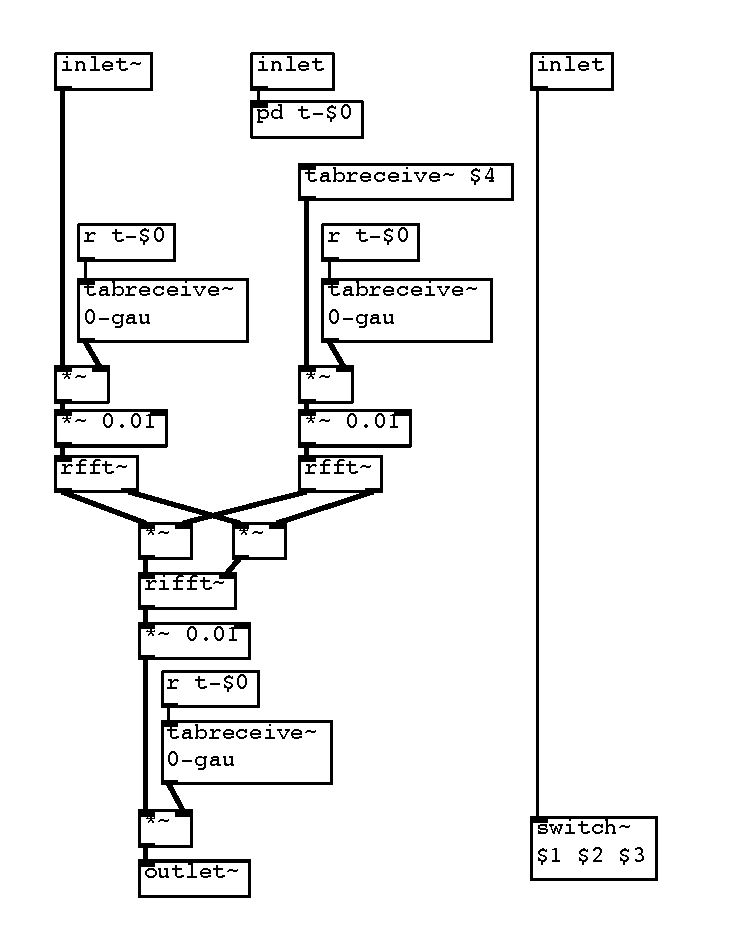
\includegraphics[width=1\columnwidth]{convolve}
    \caption{Abstraction dedicated to perform convolution. The first three arguments are 16384 16 0.25 (those of [switch\ttt]: blocksize, overlap, up/down-sampling), and the fourth is the name of the array holding the image.}
    \label{fig:convolve}
\end{figure}


\subsection{Video-based convolution}
This technique was used to generate the main sound source for the installation. It consists simply on filtered noise, where noise is Pd's [noise\ttt] (which will be mentioned later) and the filter is the array of pixels where the box with the participant's face is. The convolution takes place in the complex realm, as a multiplication of real an imaginary values of both the noise and the image array (Figure~\ref{fig:convolve}). A compromise needed to be made between frame resolution and audio computation: the image data filter dimensions in pixels was set to 128x128, and the audio block size, to 16384 samples, respectively. 

\begin{figure*}
    \centering
        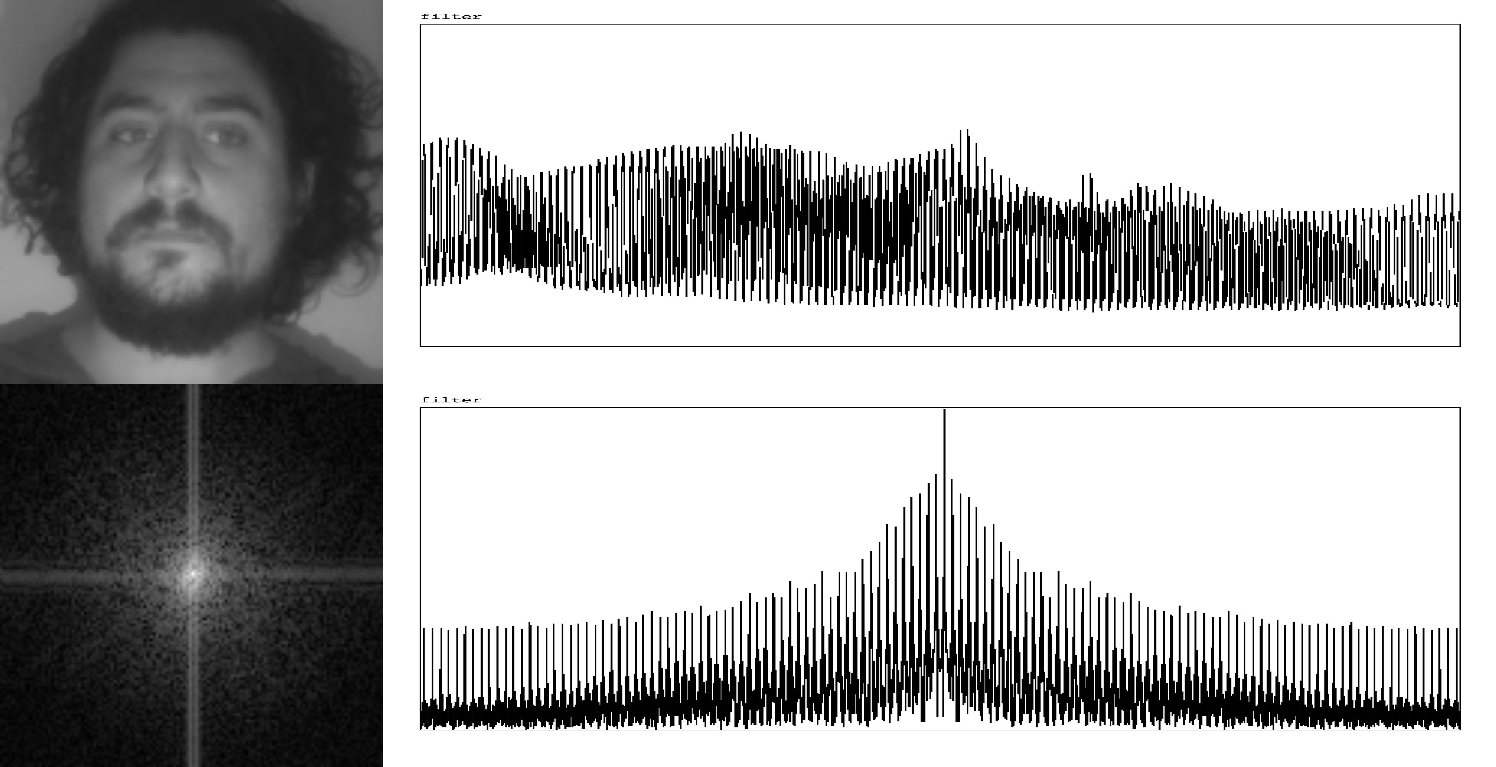
\includegraphics[width=1\linewidth]{non-and-fft}
    \caption{Left-Top: Cropped box with face. Center-Top: face array as real valued filter. Right-Top: filtered noise with real values. Left-Bottom: 2d FFT of the above cropped box with face. Center-Bottom: face array as complex valued filter. Right-Bottom: filtered noise with complex values.}
    \label{fig:non-and-fft}
\end{figure*}

On the one hand, the benefits of cropping a squared image were used in two aspects: the 2d FFT computation of the image using [pix\_fft2], and the face detection could be adjusted to the square and repositioned within the larger 640x480 image. Both of these aspects where explained above. On the other hand, the 16384 sample block of audio computation results in a fundamental pitch that is constant throughout the experience. This constant pitch was used as a performance opportunity in two ways: the first one is controlled by the participant and the second is controlled by HALLY.  

This fundamental pitch is a result of the \(2^n\) space in which memory is more efficiently handled in fast computation loops. This is to say that, in this case, pitch is determined by Pd's frequency of audio computation. Crucial to this pitch, however, is the sample rate at which it is played. Since the [switch\ttt] object allows to control these parameters, they were set so that (1) 16 overlaps (i.e. superimpositions or imbrications of the data) were performed in order to smooth the iterative quality of the rather large block-size; and (2) the convolution patch was down-sampled by a factor of 0.25, thus lowering the pitch by 2 octaves. The total latency of each block was therefore of 92.8798 milliseconds, the resulting size of each overlapping section was of 1024 samples, and the sample rate of the convolution window remained at 11025 Hz (Figure~~\ref{fig:non-and-fft}). 

The resulting pitch is of \(1/1024/44100 = 43.0664 Hz\), which is about a low F on a grand piano. This provided a more relaxed, but slow computational effort, which was suitable for the low-pitched quality of the drone-sound. Moreover, the 92.8798 milliseconds are suitable for a quiet and slower performance, since it lays within the limits of a middle-range keyboard instrument damping mechanism (as noted by \cite{oliver:drum} from\cite{askenfelt:threshold}). Furthermore, in order to counteract the response speed (and since there was enough computational space) we set the speed of the Gem window (including video capture and overall image processing) to 60 frames per second (fps). Therefore, a rapid response was present visually, preparing the participant for the listening experience by providing the ear with extra time to allow expectation to grow.

In this way, the spectrum of this fundamental pitch was \textit{played} by the participant directly. As she moved and interacted, tilted, got closer or farther, blocked or covered her face or HALLY's eyes, and in many other ways, the participant performed a spectral experience with HALLY.

\subsection{Spatialized granular synthesis} 
This is the second way the pitch was used, as controlled by HALLY. Random partials of this spectrum were used to determine the amplitude of granular sounds. These grains were understood as saliences out of the drone-like sound. 

A polyphony of maximum 32 grains were synthesized in the following way: 
\begin{itemize}
\item Step 1 : Random pitch \(f\) selected from \(32^2\) space
\item Step 2 : A pixel value \(0 > g >= 0.3\) from the image array was selected at \((ftom(f)*k) - rand(1000)\),   where \(k = 44100/16384 * 64\).  
\item Step 3 : \(g\) determined the amplitude of randomly selected envelopes from a custom selection of tables developed for \cite{camara:fdlib}
\item Step 4 : A lookup table was read by [phasor\ttt] at frequency \(f\), where the table was the array containing the face mesh (Figure~\ref{fig:ALL_FEATURES})
\item Step 5 : Finally, a random speaker assignment determined the localization, and randomized ranges from 200-5200 milliseconds determined the length of the grains.
\end{itemize}

\subsection{Did someone say Noise?}
Given that noise is the main source of \textit{otherness} that we are taking for granted in this installation, it begs the question, at this point, to wonder about the current state of noise within Pure Data. Pd's [noise\ttt] and [random] objects contain somewhat different pseudo-random number generators (PRNG), for audio and control rate respectively:\footnote{The code snippets presented here are from \url{https://github.com/pure-data/pure-data/blob/master/src/d_osc.c} and \url{https://github.com/pure-data/pure-data/blob/master/src/x_misc.c}. Both are simplified for readability, to the point that they can be understood as pseudo code.}

\subsubsection{[noise\ttt]}
The first term of the algorithm in [noise\ttt] computes the bitwise difference between \(val\) and the Mersenne Prime \(2^{31}\), then subtracts \(2^{30}\) and divides it from the result. The result is outputted at sample rate, i.e., on every iteration of the audio loop. The second term simply multiplies the previous result by \(2^{32}+1\), adding to it a \textit{magic} number 382842987, finally storing the value in memory for the next iteration.
\begin{lstlisting}
[...]
static int init = 307;
val = (init *= 1319);
[...]
((val & 0x7fffffff) - 0x40000000) / 0x40000000;
val = val * 435898247 + 382842987;
[...]
\end{lstlisting}
\subsubsection{[random]}
In the case of [random], the use of double precision instead of float precision above entails more accuracy, at the possible cost of speed. Further, like in the previous case, a seed is assigned on each instance, but here there is a seed method that enables the input of a seed (aka \(randval\), aka \(x->x\_state\)). We will discuss this further down. Moreover, the \(range\) variable adds a hard upper boundary that cuts the output at \(range-1\). The two first terms resemble [noise\ttt]'s algorithm, without the bitwise computation, with all numbers being \textit{magical} except the second term, where the seed and the range are divided by \(2^{30}\).
\begin{lstlisting}    
x->x_state = randval * 472940017 + 832416023;
nval = range * randval / 4294967296;
if (nval >= range) nval = range-1;
\end{lstlisting}
These methods can be understood as improvements on the native C function called with rand(), since it uses the Mersenne Prime, proven to be a more reliable source of randomness \cite{matsumoto:twister}. However, neither the nature of the magic number, nor the reliability of the PRNG have been determined.\footnote{The authors of this paper would like to thank, not criticize, the Pd community for this minor imprecision in the statistical processes involved. It is in these still unexplained or accidental properties where there is space for creativity and further exploration, and more importantly, for community to emerge.} The following code was simplified for readability purposes:

The flexibility of this type of PRNG is its ability to use a seed, which guarantees the a unique sequence of values for each seed. The point here is that the possibility for repetition, of two random sequences speaks of a different attitude towards art. In the audio version, as we just saw, the seed is fixed for every instance, with the comment in line 469: \textit{``seed each instance differently.  Once in a blue moon two threads could grab the same seed value.  We can live with that.''}. In fact, this means that two different instances of [noise\ttt] created simultaneously will render the same randomness. 

In the control rate version, the overuse of magic numbers comes with the comment in line 44: \textit{``this is strictly homebrew and untested''}. These lines are curiously at odds with the shift to double precision, while simultaneously in resonance with the more relaxed approach towards an artistic generation of random data, rather than strictly statistical, let alone cryptographic uses of randomness.

\subsection{Discussion}
There is still more to be said about the visual aspect of the installation (such as the automated image web search for the keyword \textit{face} each time the installation starts, which was truncated by governmental regulations in Shanghai, China), and about other kinds of interaction by a piano sustain pedal present just below the microphone stand. Similarly, we have only touched key concepts throughout this paper (sonification, immersion, robotics, tracking, spatialization, noise, feedback, etc). We will have to limit ourselves on these topics, and focus on the task at hand.

Now it is time to address the second half of the title of the installation (and the first part of this paper's): the ``spectral experience'' part. As mentioned in the introduction, our intention with this installation focused on sonifying the mechanics of brain's IFT-based perception. The constant use of FFT-s throughout the filtering or convolution seems to address this focus, given that perception according to \cite{connes:shapes} happens in the complex realm, i.e., the spectrum. However, more recent inquiries into the spectral, as understood by Timothy Morton in \cite{morton:humankind}:


\textit{`` ... spectrality is the flavor of the symbiotic real, where everything is what it is, yet nothing coincides exactly with itself.''} (P.54). The uncanniness of this flavor is what resounds with HALLY. What we termed A/V Ambience in Figure~\ref{fig:hally-human-1}, can be an instance of Morton's \textit{``symbiotic real''}. 

Following Morton's notions of interconnectedness, a new diagram can be drawn in simplification of the previous one (Figure~\ref{fig:hally-human-2}). In this last one, agency is more evident in terms of the ongoing loops that are neither aimed towards the center nor the edges, but to the condition of connection. This inevitable link between environment, human and nonhuman is understood by Morton as spectrality itself, which for him \textit{`` [is] not spirits in the divine realm, even if that realm has been relocated in the human -that's the concept of Humanity. Spectrality is nonhumans, including the 'nonhuman' aspect of ourselves.''}

\begin{figure}[htbp]
    \centering
        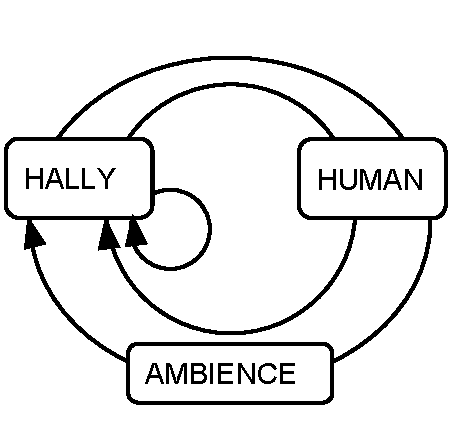
\includegraphics[width=0.5\columnwidth]{hally-human-2}
    \caption{Simplification of Figure~\ref{fig:hally-human-1}}
    \label{fig:hally-human-2}
\end{figure}

\section{Conclusions}
We have proposed an interactive, immersive, multimedia, and robotic installation, discussing the role of sound and image in the definition of the self. Sonification techniques were proposed, amongst which video-based convolution was preferred. We have aimed at non-anthropocentric approaches and introduced terms such as ecosystemic or spectrality, that aim to bring the nonhuman agency in play. Further, we have tried to bring this agency through as expression of the nonhuman self, in the anthropomorphizing HALLY and her motility and sight. The participant's exploration within this spectrality results in an uncanny and playful experience, in which she can further question these issues, and bring new aspects into play.

\bibliographystyle{abbrv}
\bibliography{hally-refs} 
\end{document}